% include file for chapter 3

\newpage \section{EXPERIMENTÁLNÍ ČÁST} \label{exp}

\subsection{Použité chemikálie a materiály} \label{materials}
Tabulka \ref{tab:chemicals} je výčtem všech použitých chemikálií.

\begin{table}[ht]
\caption{Seznam použitých chemikálií} \label{tab:chemicals}
\begin{tabularx}{\textwidth}{llp{2cm}Z}
	\Xhline{2pt} \textbf{látka} & \textbf{výrobce} & \textbf{čistota} & \textbf{H/P věty} \\ \hline
	destilovaná voda & VŠCHT & & \\
	propan-2-ol & Penta & \makecell{p.a.\\>99,8~\%} & H225, H319, H336, P210, P233, P305+P351+P338 \\
	n"-heptanol & Fluka & \makecell{p.a.\\>99,0~\%} & H319, P305+P351+P338 \\
	n-heptan & Penta & \makecell{p.a.\\>99,0~\%} & H225, H304, H315, H336, H410, P210, P243, P273, P301+P310, P331 \\
	toluen & Penta & \makecell{p.a.\\>99,0~\%} & H225, H304, H315, H336, H361d, H373, P210, P261, P280, P301+P310, P331 \\
	trichlorethylen & Spolana & \makecell{destilovaný\\99,7~\%} & H315, H317, H319, H341, H350, H412, P201, P273, P280, P302+P352, P305+P351+P338, P308+P313 \\
	kaprolaktam & Spolana & \makecell{destilovaný\\100,0~\%} & H319, H315, H332, H302, H335, P261, P280, P304+P340, P305+P351+P338, P301+P330, P403+P233 \\
	síran amonný & Lachema & \makecell{p.a.\\>99,0~\%} & H315, H319, H335, P280, P305+P351+P338 \\
	\Xhline{2pt}
\end{tabularx}
\end{table}

\subsection{Měření rovnováhy kapalina-kapalina} \label{LLE}
\textit{lorem ipsum}

\subsubsection{Aparatury a metodika experimentů} \label{LLE_exp}
K provádění experimentů na měření dat LLE byla použita aparatura znázorněná na obrázku \ref{fig:LLE_a}. Aparaturu tvoří skleněná cela, ve které je připravena fáze těžší~(1) i lehčí~(2).
Jejich disperzi zajišťuje magnetické míchadlo~(3), k udržení konstantní teploty slouží duplikátor, do nějž vstupuje~(4) a vystupuje~(5) voda z termostatu.
Těchto cel bylo k~dispozici celkem sedm. V~celách byly připraveny příslušné kapalné směsi, a~to~tak, aby objem obou fází činil zhruba 20~ml, načež bylo nastaveno míchání dostatečně intenzivní, aby vznikla jemná disperze kapalných fází.
Po zapnutí termostatu s příslušným teplotním nastavením bylo vyčkáno na ustálení teploty, poté bylo míchání ponecháno v běhu minimálně 30~min, aby se systém dostal dostatečně blízko k fázové rovnováze.
Po uplynutí této doby bylo míchání vypnuto a systém byl ponechán potřebnou dobu v klidu, aby došlo k úplnému mechanickému oddělení kapalných fází, tedy aby byly obě fáze vizuálně čiré (minimálně však 5~min).
Nakonec byly z obou fází odebrány vzorky o hmotnosti cca. 1~g, pro účely analýzy (kapitola \ref{GC}) byla vždy změřena také jejich přesná navážka na analytických vahách.

\begin{figure}[ht]
\begin{center}
	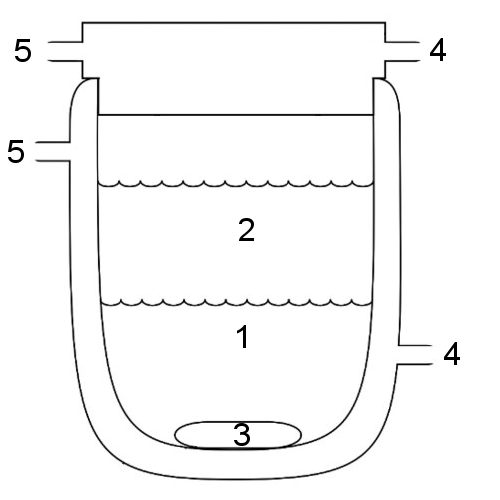
\includegraphics[width=6cm,height=6cm,keepaspectratio,]{images/LLE_cela.png}
	\caption{Aparatura na měření LLE} \label{fig:LLE_a}
\end{center}
\end{figure}

\subsubsection{Plynová chromatografie} \label{GC}
Vzorky organické i vodné fáze jak z měření dat LLE, tak z experimentů s laboratorním extraktorem (kapitola \ref{labmodel}), bylo třeba podrobit kvantitativní analýze, k čemuž byl využit plynový chromatograf (GC) Shimadzu GC-2014 vybavený plamenově ionizačním detektorem (FID).
Měřen byl pouze obsah CPL, neboť vzhledem k rozsahu měřených koncentrací lze předvídat nemísitelnost organických a vodných fází, i obsah nečistot se ukázal být pouze stopový.
Na měření obsahu SA ve vodné fázi nebyly k dispozici prostředky, takže ten byl zajištěn pouze navážkou při přípravě roztoku.
Pro účely analýzy tedy bylo předpokládáno, že vzorky organické fáze obsahují pouze CPL a solvent (TCE či TOL), zatímco vzorky kapalné fáze obsahují CPL, vodu a SA.

Stanovení obsahu CPL bylo provedeno metodou vnitřního standardu, kterým byl n"-heptanol -- do každého vzorku o známé navážce bylo na analytických vahách odváženo zhruba dvojnásobné množství standardního roztoku, který obsahuje přibližně 0,5~\% n"-heptanolu v isopropylalkoholu.
Tento roztok plní nejen funkci vnitřního standardu, ale také jako srážecí činidlo pro SA -- vzorky vodné fáze s rozpuštěnou solí by nebylo možné analyzovat, neboť by mohlo dojít k ucpání chromatografické kolony.
Po vysrážení soli tedy byla odebrána pouze kapalná fáze, která byla před nástřikem na GC ještě odstředěna na laboratorní centrifuze.

Parametry kolony a podmínky při chromatografii jsou uvedeny v tabulce \ref{tab:GC}.
Teplotní profil byl zvolen tak, aby byl retenční čas kaprolaktamu (nejméně těkavá látka z analytů) co nejnižší, a tedy aby jeho pík měl tvar co nejbližší Gaussově funkci, ale zároveň aby byly píky kaprolaktamu i n"-heptanolu dostatečně oddělené od sebe i od píků rozpouštědel.
K tomuto účelu byl přizpůsoben následující teplotní profil: 100°C po dobu 2~min, ohřev na teplotu 200°C trvající 4~min a nakonec 2~min při této teplotě.
Tabulka \ref{tab:GCtime} shrnuje přibližné hodnoty retenčních časů ($\tau_\mathrm{R}$), které byly za těchto podmínek pozorovány.
V případě, že je retenční čas zadán jako rozmezí, se jedná o pík s šikmým tvarem a jeho vrchol se proto pohybuje v závislosti na celkové ploše píku.

\begin{table}[ht]
\caption{Podmínky při analýze GC a popis kolony} \label{tab:GC}
\begin{center}
\begin{tabular}{ll}
	\Xhline{2pt}
	chromatograf & Shimadzu GC-2014\\
	ovládací software & Clarity 7.0 (DataApex)\\
	kolona & SPB-5 (Výrobce Supelco, Inc.)\\
	délka kolony & 30 m\\
	průměr kolony & 0,32 mm\\
	tloušťka filmu & 0,25 \textmu m\\
	splitovací poměr & 15\\
	objem nástřiku & 0,6 \textmu l\\ % ??? nejsem si jist, zda-li je to v mikrolitrech
	teplota injektoru & 250°C\\
	teplota detektoru & 250°C\\
	nosný plyn & He\\
	přetlak na vstupu do kolony & 72 kPa\\
	střední rychlost nosného plynu & 33,0 cm/s\\
	\Xhline{2pt}
\end{tabular}
\end{center}
\end{table}

\begin{table}[ht]
\caption{Retenční časy analytů na GC} \label{tab:GCtime}
\begin{center}
\begin{tabular}{ll}
	\Xhline{2pt}
	\textbf{Analyt} & \textbf{$\tau_\mathrm{R}$/min}\\ \hline
	propan-2-ol & 1,80\\
	toluen & 2,17\\
	n"-heptanol & 3,01\\
	kaprolaktam & 5,17--5,46\\
	\Xhline{2pt}
\end{tabular}
\end{center}
\end{table}

\subsubsection*{Zpracování chromatogramů}

Po analýze vzorku v plynovém chromatografu poskytne ovládací software chromatogram a z něj vyhodnotí různé veličiny, z nichž nejdůležitější je retenční čas, který slouží pro přiřazení píku určité látce, a plocha píku, pomocí níž lze obsah látky kvantifikovat.

Při využití metody vnitřní kalibrace lze využít vzorec \ref{eqn:GC_cal}, kde $w_\mathrm{CPL,s}$ a $w_\mathrm{Hep,s}$ značí obsah CPL a n"-heptanolu v analyzovaném vzorku (po přidání standardu), $A_\mathrm{CPL}$ a $A_\mathrm{Hep}$ značí plochy píků a $S_{^\mathrm{CPL}/_\mathrm{Hep}}$ je kalibrační koeficient kaprolaktamu vůči n"-heptanolu.
Při známých navážkách původního vzorku i standardu je tedy nejprve vypočten $w_\mathrm{Hep,s}$, následně $w_\mathrm{CPL,s}$ a nakonec lze určit $w_\mathrm{CPL}$, tedy obsah CPL v původním vzorku.

\begin{equation}
\label{eqn:GC_cal}
	w_\mathrm{CPL,s} = S_{^\mathrm{CPL}/_\mathrm{Hep}} w_\mathrm{Hep,s} \frac{A_\mathrm{CPL}}{A_\mathrm{Hep}}
\end{equation}

Pro zpracování chromatogramů však bylo nejprve nutné provést kalibraci pomocí roztoků se známým obsahem n"-heptanolu, který je při dané metodice víceméně konstantní, i kaprolaktamu, jehož obsah se může mezi měřenými vzorky řádově lišit.
Kalibrační vzorky proto byly připraveny v širokém rozsahu koncentrací, a to od 0,004--10,2~\% včetně standardu, což odpovídá 0,012--30,4~\% ve vzorku bez standardu.
Pro každý kalibrační vzorek byla určena hodnota $S_{^\mathrm{CPL}/_\mathrm{Hep}}$, a jelikož koeficient nevykazoval trend vůči obsahu CPL, byla v této práci používána průměrná hodnota.

\subsection{Měření mezifázového napětí} \label{gamma}
Pro účely sestavení matematických modelů se později ukázalo, že je třeba změřit také mezifázové napětí, neboť sice lze v literatuře nalézt vzorce na jeho odhad, jak uvádí například G.~N.~Antonov~\cite{Antonov1907} či D.~J.~Donahue a F.~E.~Bartell~\cite{Donahue1952}, ty však bývají značně nespolehlivé.
Proto bylo provedeno měření pro systém \ce{H2O}--SA--CPL--TOL, aby mohla být zjištěna závislost mezifázového napětí na koncentraci CPL ve vodné fázi.

Měření bylo provedeno pomocí kapkové metody (též známá jako stalagmometrická metoda), která je klasicky využívána pro měření povrchového napětí, lze ji však modifikovat pro měření mezifázového napětí, a to tak, že je nádoba stalagmometru naplněna vzorkem těžší fáze a kapilára je ponořena pod hladinu vzorku lehčí fáze, kde se tak tvoří rozhraní obou fází.
Postup měření je takový, že se nastaví takový vhodný tok těžší fáze, aby vznikaly kapky dostatečně pomalu, a ty jsou pak váženy v sériích čítajících alespoň dvacet kapek.
Doba mezi odtržením kapek musí být dostatečně dlouhá, jinak je měření zkresleno jevem, kdy přitékající kapalina kapku zvětší ještě při jejím odtrhávání, což vede k vyšší pozorované hmotnosti~\cite{Harkins1919}.

Mezifázové napětí~($\gamma$) lze vypočítat postupem, který popsali J.~L.~Lando a H.~T.~Oakley~\cite{Lando1967}. Vztah je uveden v rovnici~\ref{eqn:gamma}, kde $\rho_\mathrm{H}$ a $\rho_\mathrm{L}$ znamená hustotu těžší, resp. lehčí fáze, $m$ je hmotnost jedné kapky, $g$ tíhové zrychlení, $r$ poloměr kapiláry a $\Phi$ je korekční faktor, pro který autoři uvádějí empirický vztah. Ten je zde uveden v rovnici~\ref{eqn:gammaCorr}.
\begin{equation}
\label{eqn:gamma}
	\gamma = \frac{\rho_\mathrm{H} - \rho_\mathrm{L}}{\rho_\mathrm{H}} \frac{m g \Phi}{2 \pi r}
\end{equation}
\begin{equation}
\label{eqn:gammaCorr}
	\Phi = -1,044 \left(\frac{r}{\sqrt[3]{m / \rho_\mathrm{H}}}\right)^2 + 1,754 \frac{r}{\sqrt[3]{m / \rho_\mathrm{H}}} + 0,929
\end{equation}
\subsection{Laboratorní model extraktoru} \label{labmodel}
\textit{lorem ipsum}

\subsubsection{Popis aparatury} \label{labmodel_a}
\textit{lorem ipsum}

\subsubsection{Metodika experimentů} \label{labmodel_m}
o analýze jen viz kapitolu \ref{GC}
